

\lstset{
 columns=fixed,       
 numbers=left,                                        % 在左侧显示行号
 numberstyle=\tiny\color{gray},                       % 设定行号格式
 frame=none,                                          % 不显示背景边框
 backgroundcolor=\color[RGB]{245,245,244},            % 设定背景颜色
 keywordstyle=\color[RGB]{40,40,255},                 % 设定关键字颜色
 numberstyle=\footnotesize\color{darkgray},           
 commentstyle=\it\color[RGB]{0,96,96},                % 设置代码注释的格式
 stringstyle=\rmfamily\slshape\color[RGB]{128,0,0},   % 设置字符串格式
 showstringspaces=false,                              % 不显示字符串中的空格
 language=c,                                        % 设置语言
}


\chapter{模块验证与实验}
基于NB-IOT的中断应用大致分为4类,分别是固定上报类,固定控制类,移动上报类和移动控制类。不同类别的应用因为数据的实时性、数据量、部署环境等的不同,对网络以及电源的需求也不同。例如对于固定控制类,由于设备部署位置固定,常有外部电源支持,需要较强的实时性,所以对功耗需求不高,需要模块时刻保持在线状态。接下来将以一个固定上报类终端对bc35g模块进行验证。终端硬件连接如图\ref{硬件连接}
\begin{figure}[h]
    \centering
  	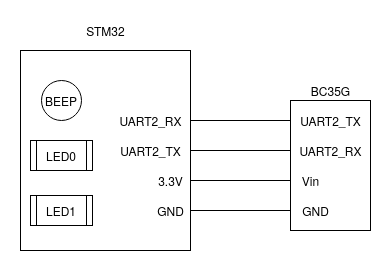
\includegraphics[width=9cm]{硬件连接.png}
	\caption{硬件连接}
	\label{硬件连接}
\end{figure}

\section{总体设计}


\section{华为云平台应用开发}
华为 OceanConnect物联网平台作为一个连接业务应用和物联网设备的中间层,提供了海量设备接入管理,屏蔽复杂的设备接口,可以快速构筑物联网应用。
%\begin{figure}[h]
%    \floatcontinue
%	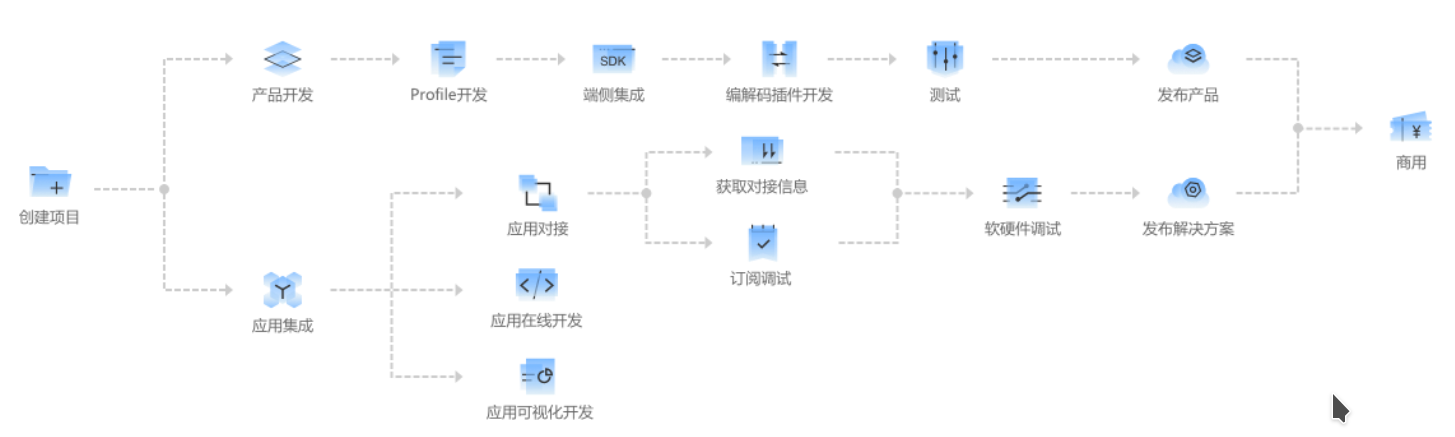
\includegraphics[width=20cm]{oc流程.png}
%	\caption{oc流程}
%	\label{oc流程}
%\end{figure}

\subsection{定义产品}
产品是指一类具备相同能力和特征的设备,一个产品包含产品模型、编解码插件等资源。选用CoAp协议,由于使用JSON的数据格式对能耗消耗太大,不适用于物联网设备,所以选用二进制码流的数据格式,通过开发编解码插件解析。
\begin{figure}[H]
    \centering
	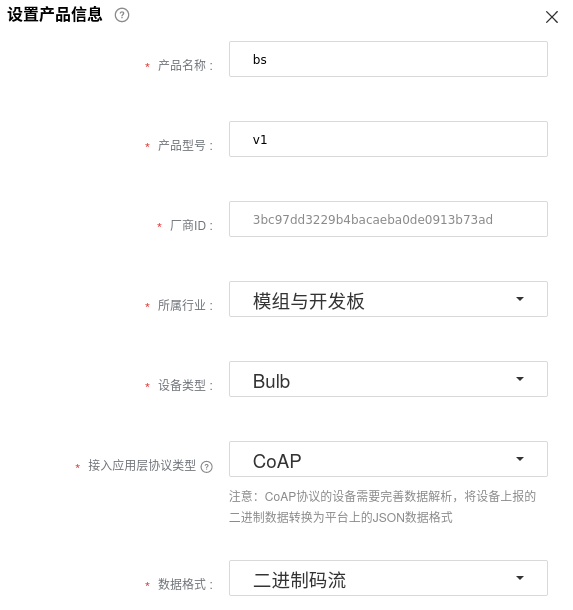
\includegraphics[width=9cm]{oc产品.png}
	\caption{oc产品定义}
	\label{oc产品}
\end{figure}


\subsection{定义profile与编解码插件}
profile是描述产品设备信息的文件,定义了设备与应用服务器交互的字段及格式。其主要包含产品信息、服务能力以及维护能力。以控制开发板LED灯相关的profile信息为例,定义profile如下:
\begin{table}[h]
\caption{profile格式}
\begin{tabular}{|c|c|c|c|c|}
\toprule
\multicolumn{5}{|l|}{属性列表} \\
\hline
属性名称 & 类型 & 取值 & \multicolumn{2}{|c|}{描述}  \\
\hline
led0 & int & 0~1 & \multicolumn{2}{|l|}{0:led0关闭 1:led0开启} \\
\hline
led1 & int & 0~1 & \multicolumn{2}{|l|}{0:led1关闭 1:led1开启} \\
\hline
beep & int & 0~1 & \multicolumn{2}{|l|}{0:蜂鸣器关闭 1:蜂鸣器开启} \\
\toprule
\multicolumn{5}{|l|}{命令列表} \\
\hline
命令名称 & 字段属性 & 字段名 & 取值 & 描述 \\
\hline
\multirow{2}{*}{set\_resouce} & 请求 & num & 1-3 & 资源编号 \\
\cmidrule{2-5}
&请求&state&0-1&资源状态 \\
\hline
query\_resouce & 请求 & num & 1-3 & 资源编号 \\
\hline
\bottomrule
\end{tabular}
\label{tablea}
\end{table}

二进制数据格式需要编解码插件才能解析,在oc平台上设置好profile 文件后,将相应属性值与消息模板中的字段相连接,oc平台将会自动生成编解码器,在stm32中也根据消息模板对消息进行编解码。

\begin{table}[h]
\caption{消息模板}
\begin{tabular}{|c|c|c|c|c|c|}
\toprule
消息类型 & 字段名称 & 数据类型 & 偏移量 & 字段解释 & 消息解释 \\
\hline
\multirow{4}{*}{resource\_info} & messageId & uint8 & 0-1 & 消息类型编号:2 & \multirow{4}{*}{模块上报消息} \\
\cmidrule{2-5}
& led0 & uint8 & 1-2 & led0 状态 & \\
\cmidrule{2-5}
& led1 & uint8 & 2-3 & led1 状态 & \\
\cmidrule{2-5}
& beep & uint8 & 3-4 & beep 状态 & \\
\hline
\multirow{3}{*}{set\_resource} & messageId & uint8 & 0-1 & 消息类型编号:0 & \multirow{3}{*}{模块控制消息} \\
\cmidrule{2-5}
& num & uint8 & 1-2 & 需要控制的资源编号 & \\
\cmidrule{2-5}
& state & uint8 & 2-3 & 资源状态 & \\
\hline
\multirow{3}{*}{query\_resource} & messageId & uint8 & 0-1 & 消息类型编号:1 & \multirow{3}{*}{触发模块上报} \\
\cmidrule{2-5}
& num & uint8 & 1-2 & 需要上报的资源编号 & \\
\bottomrule
\end{tabular}
\label{tablea}
\end{table}


\subsection{接入设备}
通过串口连接设备,使用AT+CSGB=1命令查询设备IMEI号,在oc平台上增加设备,并从oc平台获取CoAP接入地址\ref{oc接入方式},以作为NCDP参数,华为云平台上的设置就完成了。
\begin{figure}[h]
	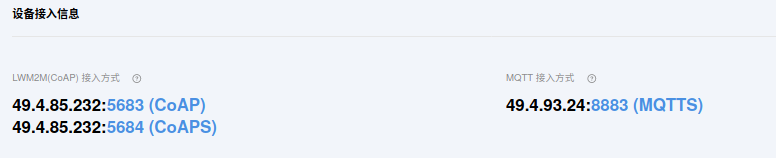
\includegraphics[width=15cm]{oc接入方式.png}
	\caption{oc接入方式}
	\label{oc接入方式}
\end{figure}


\section{stm32终端开发}
stm32终端选择一块搭载stm32f103zet的开发板,板载4组串口,第一组可用于USB通信。本次验证使用到其中第二组串口,对应引脚为PA2和PA3。使用无源蜂鸣器及一组LED灯,作为控制量,对应引脚为PB8,PB5,PE5。使用key0-3,对应引脚为PE2,PE3,PE4。

key0-3用作外部中断输入,分别对应模块的初始化、重连和退网,led和无源蜂鸣器用作被操控的系统资源,串口用于控制通信模块。


\subsection{串口DMA通信}

stm32开发板控制bc35g模块是通过串口的方式,bc35g串口比特率为9600。为了接收变长的串口数据,可以有以下几种方式:

BC35G模块串口传输数据以'lr cr'为分隔符,以软件的方式,设置超时接收固定长度并以'lr cr'分割,放入缓冲区中。由于模块涉及网络操作等原因,不同AT指令的响应时间有很大差距,所以超时时间不好确定,同时由于MCU等待模块输入,对效率影响较大。

利用定时器中断方式可以解决超时时间设置的问题。一个字节的数据有 起始位+数据+结束位共10位,在模块串口比特率为9600的情况下,传输一个字节需要104us。同时由于两组数据之间需要间隔3.5字符,可以设置定时器中断为5ms。在串口接收中断服务函数中开启定时器中断,每接收一个字符则重置定时器,当定时器超时时可以认为一组数据接收完毕,在定时器中断函数中将接收到的数据放入缓存中。但是由于是一字节一字节接收,而且MCU仍然参与接收过程,所以效率仍有提升必要。

为了进一步提升效率,可以使用DMA方式接收数据。为了区分两组数据,开启总线空闲中断,当DMA传输完毕时触发总线空闲中断,在总线空闲中断中标记数据就绪。DMA方式能获得更好的效率。

\begin{lstlisting}
/* uart.c
* 检测空闲中断,标记缓存数据可用
*/

uint8_t UART2DATAREADY = 0;
uint8_t UART2RXBUFFER[UART_BUFFER_SIZE];

void USER_UART_IRQHandler(UART_HandleTypeDef *huart) {
    if (huart == &huart2) {
        if (RESET != __HAL_UART_GET_FLAG(&huart2, 
                UART_FLAG_IDLE)) {
            __HAL_UART_CLEAR_IDLEFLAG(&huart2);
            HAL_UART_DMAStop(&huart2);
            UART2DATAREADY = UART_BUFFER_SIZE - 
            __HAL_DMA_GET_COUNTER(&hdma_usart2_rx);
        }
    }
}

/* nbiot.c
* 封装AT指令执行模块,接收模块串口回传数据
*/
func NBCommand(AT_command) {
    UART_Transmit(AT_command);
    HAL_UART_Receive_DMA(&huart2, 
                        UART2RXBUFFER, 
                        UART_BUFFER_SIZE);
    Delay(100); //降低UART2DATAREADY datarace概率
    while (!UART2DATAREADY) {
        HAL_Delay(50);
    }
    data=UART2RXBUFFER;
    UART2DATAREADY = 0;
    return data;
}

\end{lstlisting}

\subsection{初始化及入网}
BC35G模块初始化需要设置云平台CoAP协议接入地址,根据USIM卡设置运营商频段。同时为了达到固定控制类应用对时延的要求,也需要关闭省电模式。为了更清晰简单的与服务端交互数据,也许关闭串口数据自动上报。最终触发入网并查询入网状态,需要执行的流程及AT指令如图\ref{入网流程}

\begin{figure}[H]
    \centering
	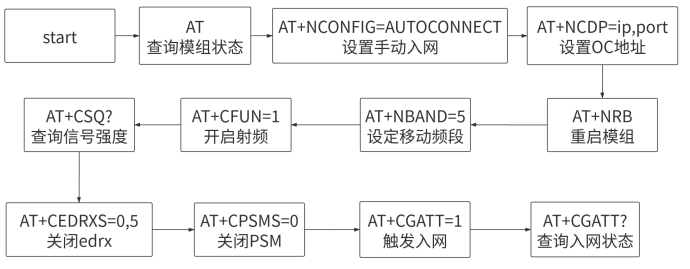
\includegraphics[width=13cm]{入网流程.png}
	\caption{入网流程}
	\label{入网流程}
\end{figure}


如果入网失败,可以尝试重连,重练操作序列如图\ref{入网重试}

\begin{figure}[H]
    \centering
	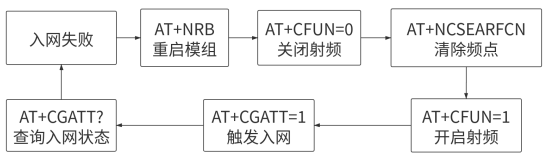
\includegraphics[width=13cm]{入网重试.png}
	\caption{入网重试}
	\label{入网重试}
\end{figure}

当设备不处于第一次开机的流程,入网操作只需要打开射频功能以及触发入网,如图

\subsection{模组通信}

bc35g模块涉及消息发送与接收的有如下四个命令:
\begin{table}[h]
\caption{bc35g模块收发命令}
\begin{tabular}{|c|c|}
\toprule
命令 & 描述 \\
AT+NMGS=<length>,<data> & \makecell[l]{data为16进制数据,length为data长度,\\用于向IOT平台发送数据} \\
AT+NIMI=0/1 & \makecell[l]{关闭/开启自动上报,模块接收到消息是会\\自动发往串口} \\
AT+NQMGR & \makecell[l]{查询自开机以来接收到的消息状态} \\
AT+NMGR & \makecell[l]{读取缓存中最早一条未被未被处理的消息} \\
\bottomrule
\end{tabular}
\label{tablea}
\end{table}

如果开启自动上报,则服务器下发内容有可能与串口控制消息重叠,需要消耗额外资源去提取。同时由于固定控制类应用对延时要求较高,所以关闭自动上报,定时轮询缓存中是否有接收到新消息。

\begin{lstlisting}

//nbiot.c
func readMsg(){
    received=NBCommand("AT+NQMGR")
    for read to received{
        data+=NBCommand("AT+NMGR")
    }
    data+="command_end"
    read=received;
    return data;
}

//main.c
while(1){
    Delay(1000);
    data=readMsg();
    process(data);
}
\end{lstlisting}


\subsection{退网关机}

当设备关机时需要释放与运营商的连接,须执行以下序列\ref{模块关机}
\begin{figure}[H]
    \centering
	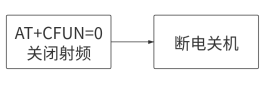
\includegraphics[width=7cm]{模块关机.png}
	\caption{模块关机}
	\label{模块关机}
\end{figure}

\section{验证过程以及结论}

\section{本章小结}

本章通过简单模拟一个固定控制类应用,在STM32开发板上实现对BC35G模块的通信控制,通过CoAP协议,完成查询、上报、控制资源状态三种消息类型的传输,验证了BC35G模块的功能